\documentclass[10pt]{book}
% mathematics and figures
\usepackage{graphicx}
\usepackage{amsmath}
\usepackage{amssymb}
\usepackage{capt-of}
% plot
\usepackage{pgfplots}
\usepackage{array}
\usepackage{fontspec}
\usepackage[Sinhala,Latin]{ucharclasses}
\setmainfont{Noto Serif}[NFSSFamily=standardserif]
\setsansfont{Noto Sans}[NFSSFamily=standardsans]

\newfontfamily\sinhalaserif{Noto Serif Sinhala}[
  NFSSFamily=sinhalaserif,
]
\newfontfamily\sinhalasans{Noto Sans Sinhala}[
  NFSSFamily=sinhalasans,
]

\setDefaultTransitions{\switchto{standard}}{}
\setTransitionTo{Sinhala}{\switchto{sinhala}}

\ExplSyntaxOn
\NewDocumentCommand{\switchto}{m}
 {
  \str_case_e:vnF {f@family}
   {
    { standardsans } { \fontfamily{#1sans}\selectfont }
    { sinhalasans } { \fontfamily{#1sans}\selectfont }
   }
   { \fontfamily{#1serif}\selectfont }
 }
\cs_generate_variant:Nn \str_case_e:nnF { v }
\cs_generate_variant:Nn \tl_show:n { v }
\ExplSyntaxOff


\renewcommand\contentsname{පටුන}
\renewcommand\listfigurename{රූපාවලිය}
\renewcommand\listtablename{වගුවාවලිය}
\renewcommand\bibname{උපුටන}
\renewcommand\indexname{සූචිය}
\renewcommand\figurename{රූපය}
\renewcommand\tablename{වගුව}
\renewcommand\partname{කොටස}
\renewcommand\chaptername{පරිච්ඡේදය}
\renewcommand\appendixname{උපග්‍රන්ථය}
\def\today{\ifcase\month\or
  ජනවාරි\or පෙබරවාරි\or මාර්තු\or අප්‍රේල්\or මැයි\or ජූනි\or
  ජූලි\or අගෝස්තු\or සැප්තැම්බර්\or ඔක්තෝම්බර්\or නොවැම්බර්\or දෙසැම්බර්\fi
  \space\number\day, \number\year}

\tolerance=1
\emergencystretch=\maxdimen
\hyphenpenalty=10000
\hbadness=10000

\title{\bf ශුද්ධ වූ බයිබලය}
\author{ශුද්ධ වූ සභාව}


\begin{document}                        
\frontmatter                            
\maketitle                              
\tableofcontents                        
\listoffigures
\listoftables
\mainmatter                             
\part{පැරණි ගිවිසුම}                   
\chapter{උත්පත්ති}                
වක්‍රය {ආරම්භයේ} දී සියල්ල අඳුරු විය. දෙවියන් වහන්සේ ආලෝකය වේවා යි වදාළ  සේක.පටන්ගැන්මෙහිදී දෙවියන්වහන්සේ අහසත් පොළොවත් මැවූසේක. 2පොළොව වනාහි පාළුව හිස්ව තිබුණාය; ගැඹුර පිට අන්ධකාරය විය. දෙවියන්වහන්සේගේ ආත්මය ජල මතුයෙහි හැසිරෙමින් සිටිසේක. 3දෙවියන්වහන්සේ: එළිය වේවයි කීසේක; එවිට එළිය විය. 4එළිය යහපත් බව දෙවියන්වහන්සේ දුටුසේක. 5දෙවියන්වහන්සේ අන්ධකාරයෙන් එළිය වෙන් කොට එළියට දවාලය කියාද අන්ධකාරයට රාත්‍රියය කියාද නම් තැබූසේක. සවස විය, උදය විය, ඒ එක දවසක්ය. 6දෙවියන්වහන්සේ: ජල මධ්‍යයෙහි අවකාශයක් වේවා, එය කරණකොට ගෙන ජලය ජලයෙන් වෙන්වේවයි කීසේක. 7දෙවියන්වහන්සේ අවකාශය සාදා අවකාශයට උඩින් තිබුණු ජලයෙන් අවකාශයට යටින් තිබුණු ජලය වෙන්කළසේක; ඒ එසේ විය. 8දෙවියන්වහන්සේ අවකාශයට අහසය කියා නම් තැබූසේක. සවස විය, උදය විය, ඒ දෙවෙනි දවසක්ය. 9දෙවියන්වහන්සේ: අහසට යටින් තිබෙන ජලය එක් තැනකට රැස් වේවා, වියළි බිම පෙනේවයි කීසේක. ඒ එසේ විය. 10දෙවියන්වහන්සේ: වියළි බිමට පොළොවය කියාද රැස්වූ ජලයට මුහුදය කියාද නම් තැබූසේක. දෙවියන්වහන්සේ ඒ යහපත් බව දුටුසේක. 11දෙවියන්වහන්සේ: පොළොව වනාහි තෘණද බීජ උපදවන පලාද ඒ ඒ වර්ග ලෙස ඵල දරන බීජ සහිත ඵල වෘක්ෂද පොළොව පිට හටගන්වාවයි කීසේක. ඒ එසේවිය. 12තෘණද ඒ ඒ වර්ග ලෙස බීජ උපදවන පලාද ඒ ඒ වර්ග ලෙස බීජ සහිත ඵලදරන වෘක්ෂද පොළොවෙන් හටගත්තේය. දෙවියන්වහන්සේ ඒ යහපත් බව දුටුසේක. 13සවස විය, උදය විය, ඒ තුන්වෙනි දවසක්ය. 14දෙවියන්වහන්සේ: රාත්‍රියෙන් දවාල වෙන් කිරීමට අහස්තලයෙහි ආලෝකයෝ වෙත්වා, ඒවා ලකුණු පිණිසද සෘතු පිණිසද දවස් පිණිසද අවුරුදු පිණිසද වෙත්වා, 15පොළොවට එළිය දීමට ඒවා අහස්තලයෙහි ආලෝකයන් පිණිස වෙත්වයි කීසේක. ඒ එසේ විය. 16දෙවියන්වහන්සේ මහත් ආලෝක දෙක සෑදූසේක; වඩා මහත් ආලෝකය දිවාභාගය කෙරෙහි අධිපතිකම් කරන පිණිසය, කුඩා ආලෝකය රාත්‍රිභාගය කෙරෙහි අධිපතිකම් කරන පිණිසය. උන්වහන්සේ තාරකාද සෑදූසේක. 17පොළොවට එළිය දෙන පිණිසත් දවාල කෙරෙහිද රාත්‍රිය කෙරෙහිද අධිපතිකම් කරන පිණිසත් 18අන්ධකාරයෙන් එළිය වෙන්කරන පිණිසත් දෙවියන්වහන්සේ ඒවා අහස් තලයෙහි තැබූසේක. දෙවියන්වහන්සේ ඒ යහපත් බව දුටුසේක. 19සවස විය, උදය විය, ඒ සතරවෙනි දවසක්ය. 20දෙවියන්වහන්සේ: ජලය වනාහි එහි හැසිරෙන ජීවමාන සත්ත්වයන් බොහෝ කොට හටගන්වාවා, පක්ෂීහු පොළොවට උඩින් ආකාශ කුක්ෂීයෙහි පියාසර කෙරෙත්වයි කීසේක. 21තවද දෙවියන්වහන්සේ ඉතා මහත් ජලචර සත්ත්වයන්ද ඒ ඒ වර්ගලෙස ජලයෙහි බොහෝ සෙයින් හටගත්තාවූ එහි හැසිරෙන පණ ඇති සියලු සත්ත්වයන්ද ඒ ඒ වර්ග ලෙස පියාපත් ඇති සියලු පක්ෂීන්ද මැවූසේක. දෙවියන්වහන්සේ ඒ යහපත් බව දුටුසේක. 22දෙවියන්වහන්සේ උන්ට ආශීර්වාදකොට: තොපි සඵලව බෝවෙමින් මුහුදු ජලය පුරා පැතිර සිටිව්, පක්ෂීහුද පොළොවෙහි බෝවෙත්වයි කීසේක. 23සවස විය, උදය විය, ඒ පස්වෙනි දවසක්ය. 24දෙවියන්වහන්සේ: පොළොව වනාහි ඒ ඒ වර්ග ලෙස තිරිසනුන්ද බඩගා යන ජාතීන්ද පොළොවේ මෘගයන්ද යන ජීවමාන සත්ත්වයන් ඒ ඒ වර්ග ලෙස හට ගන්වාවයි කීසේක. ඒ එසේ විය. 25දෙවියන්වහන්සේ ඒ ඒ වර්ග ලෙස පොළොවේ මෘගයන්ද ඒ ඒ වර්ග ලෙස සිව්පාවුන්ද ඒ ඒ වර්ග ලෙස භූමියෙහි බඩගා යන සියලු සතුන්ද සෑදූසේක. දෙවියන්වහන්සේ ඒ යහපත් බව දුටුසේක. 26තවද දෙවියන්වහන්සේ: අපගේ ස්වරූපයෙන් අපගේ සමානත්වය ලෙස මනුෂ්‍යයා සාමැවීම, උදය විය, ඒ සවෙනි දවසක්ය. 
 
\section{මැවීම}                  
පටන්ගැන්මෙහිදී දෙවියන්වහන්සේ අහසත් පොළොවත් මැවූසේක. 2පොළොව වනාහි පාළුව හිස්ව තිබුණාය; ගැඹුර පිට අන්ධකාරය විය. දෙවියන්වහන්සේගේ ආත්මය ජල මතුයෙහි හැසිරෙමින් සිටිසේක. 3දෙවියන්වහන්සේ: එළිය වේවයි කීසේක; එවිට එළිය විය. 4එළිය යහපත් බව දෙවියන්වහන්සේ දුටුසේක. 5දෙවියන්වහන්සේ අන්ධකාරයෙන් එළිය වෙන් කොට එළියට දවාලය කියාද අන්ධකාරයට රාත්‍රියය කියාද නම් තැබූසේක. සවස විය, උදය විය, ඒ එක දවසක්ය. 6දෙවියන්වහන්සේ: ජල මධ්‍යයෙහි අවකාශයක් වේවා, එය කරණකොට ගෙන ජලය ජලයෙන් වෙන්වේවයි කීසේක. 7දෙවියන්වහන්සේ අවකාශය සාදා අවකාශයට උඩින් තිබුණු ජලයෙන් අවකාශයට යටින් තිබුණු ජලය වෙන්කළසේක; ඒ එසේ විය. 8දෙවියන්වහන්සේ අවකාශයට අහසය කියා නම් තැබූසේක. සවස විය, උදය විය, ඒ දෙවෙනි දවසක්ය. 9දෙවියන්වහන්සේ: අහසට යටින් තිබෙන ජලය එක් තැනකට රැස් වේවා, වියළි බිම පෙනේවයි කීසේක. ඒ එසේ විය. 10දෙවියන්වහන්සේ: වියළි බිමට පොළොවය කියාද රැස්වූ ජලයට මුහුදය කියාද නම් තැබූසේක. දෙවියන්වහන්සේ ඒ යහපත් බව දුටුසේක. 11දෙවියන්වහන්සේ: පොළොව වනාහි තෘණද බීජ උපදවන පලාද ඒ ඒ වර්ග ලෙස ඵල දරන බීජ සහිත ඵල වෘක්ෂද පොළොව පිට 

\subsection{කරුණාව}
හටගන්වාවයි කීසේක. ඒ එසේවිය. 12තෘණද ඒ ඒ වර්ග ලෙස බීජ උපදවන පලාද ඒ ඒ වර්ග ලෙස බීජ සහිත ඵලදරන වෘක්ෂද පොළොවෙන් හටගත්තේය. දෙවියන්වහන්සේ ඒ යහපත් බව දුටුසේක. 13සවස විය, උදය විය, ඒ තුන්වෙනි දවසක්ය. 14දෙවියන්වහන්සේ: රාත්‍රියෙන් දවාල වෙන් කිරීමට අහස්තලයෙහි ආලෝකයෝ වෙත්වා, ඒවා ලකුණු පිණිසද සෘතු පිණිසද දවස් පිණිසද අවුරුදු පිණිසද වෙත්වා, 15පොළොවට එළිය දීමට ඒවා අහස්තලයෙහි ආලෝකයන් පිණිස වෙත්වයි කීසේක. ඒ එසේ විය. 16දෙවියන්වහන්සේ මහත් ආලෝක දෙක සෑදූසේක; වඩා මහත් ආලෝකය දිවාභාගය කෙරෙහි අධිපතිකම් කරන පිණිසය, කුඩා ආලෝකය රාත්‍රිභාගය කෙරෙහි අධිපතිකම් කරන පිණිසය. උන්වහන්සේ තාරකාද සෑදූසේක.

\subsubsection{ධෛර්යය}
 17පොළොවට එළිය දෙන පිණිසත් දවාල කෙරෙහිද රාත්‍රිය කෙරෙහිද අධිපතිකම් කරන පිණිසත් 18අන්ධකාරයෙන් එළිය වෙන්කරන පිණිසත් දෙවියන්වහන්සේ ඒවා අහස් තලයෙහි තැබූසේක. දෙවියන්වහන්සේ ඒ යහපත් බව දුටුසේක. 19සවස විය, උදය විය, ඒ සතරවෙනි දවසක්ය. 20දෙවියන්වහන්සේ: ජලය වනාහි එහි හැසිරෙන ජීවමාන සත්ත්වයන් බොහෝ කොට හටගන්වාවා, පක්ෂීහු පොළොවට උඩින් ආකාශ කුක්ෂීයෙහි පියාසර කෙරෙත්වයි කීසේක. 21තවද දෙවියන්වහන්සේ ඉතා මහත් ජලචර සත්ත්වයන්ද ඒ ඒ වර්ගලෙස ජලයෙහි බොහෝ සෙයින් හටගත්තාවූ එහි හැසිරෙන පණ ඇති සියලු සත්ත්වයන්ද ඒ ඒ වර්ග ලෙස පියාපත් ඇති සියලු පක්ෂීන්ද මැවූසේක. දෙවියන්වහන්සේ ඒ යහපත් බව දුටුසේක. 22දෙවියන්වහන්සේ උන්ට ආශීර්වාදකොට: තොපි සඵලව බෝවෙමින් මුහුදු ජලය පුරා පැතිර සිටිව්, පක්ෂීහුද පොළොවෙහි බෝවෙත්වයි කීසේක. 23සවස විය, උදය විය, ඒ පස්වෙනි දවසක්ය.
 
\paragraph{දේව භක්තිය} 
  \textsf{24දෙවියන්වහන්සේ: පොළොව වනාහි ඒ ඒ වර්ග ලෙස තිරිසනුන්ද බඩගා යන ජාතීන්ද පොළොවේ මෘගයන්ද යන ජීවමාන සත්ත්වයන් (ඒ ඒ වර්ග ලෙස හට ගන්වාවයි කීසේක.) ඒ එසේ විය. 25දෙවියන්වහන්සේ ඒ ඒ වර්ග ලෙස පොළොවේ මෘගයන්ද ඒ ඒ වර්ග ලෙස සිව්පාවුන්ද ඒ ඒ වර්ග ලෙස භූමියෙහි බඩගා යන සියලු සතුන්ද සෑදූසේක.} \\

\begin{center}
\begin{tikzpicture}
    \begin{axis}[domain=0:1,
    xlabel=$\epsilon~~\text{ වෙනස}$,
    ylabel=$d(\epsilon)~~\text{ පරතරය}$,
    xtick={0,1},
	xticklabels={$0$, $1$},
	ytick={0,sqrt(6)/3},
	yticklabels={$0$, $\sqrt6/3$},
	grid=both]
    \addplot[mark=none, samples=100, red] function {sqrt(6)*(1-x)/3};
    \end{axis}
\end{tikzpicture}
\captionof{figure}{මුළු පොළෝතලයෙහි ඇති බීජ}
\end{center}
 
දෙවියන්වහන්සේ ඒ යහපත් බව දුටුසේක. 26තවද දෙවියන්වහන්සේ: අපගේ ස්වරූපයෙන් අපගේ සමානත්වය ලෙස මනුෂ්‍යයා සාදම්හ; ඔව්හු මුහුදේ මත්ස්‍යයන් කෙරෙහිද ආකාශයේ පක්ෂීන් කෙරෙහිද තිරිසනුන් කෙරෙහිද මුළු පොළොව කෙරෙහිද පොළොව පිට බඩගා යන සියල්ලන් කෙරෙහිද ආණ්ඩුකෙරෙත්වයි කීසේක. 27දෙවියන්වහන්සේ තමන් ස්වරූපයෙන් මනුෂ්‍යයා මැවුසේක, දෙවියන්වහන්සේගේ ස්වරූපයෙන් ඔහු මැවුසේක; පුරුෂයාද ස්ත්‍රියද කොට ඔවුන් මැවූසේක. 28දෙවියන්වහන්සේ ඔවුන්ට ආශීර්වාදකළසේක;

\begin{equation}
\nabla c=\left({\partial c\over \partial a}, {\partial c\over \partial b}\right)=\left({1\over 2}\sqrt{b\over a},{1\over 2}\sqrt{a\over b}\right)
\end{equation}

 දෙවියන්වහන්සේ ඔවුන්ට කියනසේක්: නුඹලා බෝවී වැඩිවෙමින් පොළොව පූර්ණකොට ඒක යටත්කරගනිව්; මුහුදේ මත්ස්‍යයන් කෙරෙහිද ආකාශයේ පක්ෂීන් කෙරෙහිද පොළොව පිට හැසිරෙන සියලු සතුන් කෙරෙහිද අධිපතිකම් කරව්යයි කීසේක. 29තවද දෙවියන්වහන්සේ: බලව, මුළු පොළෝතලයෙහි ඇති බීජ දරන සියලු පලාද බීජ දරන ඵල ඇති සියලු වෘක්ෂයන්ද නුඹලාට දුනිමි; එය නුඹලාට ආහාර පිණිස වන්නේය. 30පොළොවේ සියලු මෘගයන්ටත් ආකාශයේ සියලු පක්ෂීන්ටත් පොළොව පිට බඩගා යන පණ ඇති (සියලු සතුන්ටත් ආහාර පිණිස) (test)සියලු නිල් පලා දුනිමියි කීසේක. ඒ එසේ විය. 31දෙවියන්වහන්සේ තමන් සෑදූ සියල්ලම දුටුසේක, බලව ඒ ඉතා යහපත්ව තිබුණේය. සවස විය, උදය විය, ඒ සවෙනි දවසක්ය. 
 
\part{අලුත් ගිවිසුම}           
\chapter{මතෙව්}                
වක්‍රය {ආරම්භයේ} දී සියල්ල අඳුරු විය. දෙවියන් වහන්සේ ආලෝකය වේවා යි වදාළ  සේක.පටන්ගැන්මෙහිදී දෙවියන්වහන්සේ අහසත් පොළොවත් මැවූසේක. 2පොළොව වනාහි පාළුව හිස්ව තිබුණාය; ගැඹුර පිට අන්ධකාරය විය. දෙවියන්වහන්සේගේ ආත්මය ජල මතුයෙහි හැසිරෙමින් සිටිසේක. 3දෙවියන්වහන්සේ: එළිය වේවයි කීසේක; එවිට එළිය විය. 4එළිය යහපත් බව දෙවියන්වහන්සේ දුටුසේක. 5දෙවියන්වහන්සේ අන්ධකාරයෙන් එළිය වෙන් කොට එළියට දවාලය කියාද අන්ධකාරයට රාත්‍රියය කියාද නම් තැබූසේක. සවස විය, උදය විය, ඒ එක දවසක්ය. 6දෙවියන්වහන්සේ: ජල මධ්‍යයෙහි අවකාශයක් වේවා, එය කරණකොට ගෙන ජලය ජලයෙන් වෙන්වේවයි කීසේක. 7දෙවියන්වහන්සේ අවකාශය සාදා අවකාශයට උඩින් තිබුණු ජලයෙන් අවකාශයට යටින් තිබුණු ජලය වෙන්කළසේක; ඒ එසේ විය. 8දෙවියන්වහන්සේ අවකාශයට අහසය කියා නම් තැබූසේක. සවස විය, උදය විය, ඒ දෙවෙනි දවසක්ය. 9දෙවියන්වහන්සේ: අහසට යටින් තිබෙන ජලය එක් තැනකට රැස් වේවා, වියළි බිම පෙනේවයි කීසේක. ඒ එසේ විය. 10දෙවියන්වහන්සේ: වියළි බිමට පොළොවය කියාද රැස්වූ ජලයට මුහුදය කියාද නම් තැබූසේක. දෙවියන්වහන්සේ ඒ යහපත් බව දුටුසේක. 11දෙවියන්වහන්සේ: පොළොව වනාහි තෘණද බීජ උපදවන පලාද ඒ ඒ වර්ග ලෙස ඵල දරන බීජ සහිත ඵල වෘක්ෂද පොළොව පිට හටගන්වාවයි කීසේක. ඒ එසේවිය. 12තෘණද ඒ ඒ වර්ග ලෙස බීජ උපදවන පලාද ඒ ඒ වර්ග ලෙස බීජ සහිත ඵලදරන වෘක්ෂද පොළොවෙන් හටගත්තේය. දෙවියන්වහන්සේ ඒ යහපත් බව දුටුසේක. 13සවස විය, උදය විය, ඒ තුන්වෙනි දවසක්ය. 14දෙවියන්වහන්සේ: 


\begin{table}[!hbt]
\begin{center}
\caption{රූපය~\ref{fig:graph} හි අදෘශ්‍යමාන සංකූලතා}
\label{tab:data}
\begin{tabular}{|l|c|r|}
\hline
උස &  පළල & දිග \\
\hline
-5 & -5.39 & -5.42\\
-4 & -5.8 & -5.78\\
-3 & -6.25 & -6.21\\
-2 & -6.7 & -6.71\\
-1 & -7.28 & -7.3\\
\hline
\end{tabular}
\end{center}
\end{table}

රාත්‍රියෙන් දවාල වෙන් කිරීමට අහස්තලයෙහි ආලෝකයෝ වෙත්වා, ඒවා ලකුණු පිණිසද සෘතු පිණිසද දවස් පිණිසද අවුරුදු පිණිසද වෙත්වා, 15පොළොවට එළිය දීමට ඒවා අහස්තලයෙහි ආලෝකයන් පිණිස වෙත්වයි කීසේක. ඒ එසේ විය. 16දෙවියන්වහන්සේ මහත් ආලෝක දෙක සෑදූසේක; වඩා මහත් ආලෝකය දිවාභාගය කෙරෙහි අධිපතිකම් කරන පිණිසය, කුඩා ආලෝකය රාත්‍රිභාගය කෙරෙහි අධිපතිකම් කරන පිණිසය. උන්වහන්සේ තාරකාද සෑදූසේක. 17පොළොවට එළිය දෙන පිණිසත් දවාල කෙරෙහිද රාත්‍රිය කෙරෙහිද අධිපතිකම් කරන පිණිසත් 18අන්ධකාරයෙන් එළිය වෙන්කරන පිණිසත් දෙවියන්වහන්සේ ඒවා අහස් තලයෙහි තැබූසේක. දෙවියන්වහන්සේ ඒ යහපත් බව දුටුසේක. 19සවස විය, උදය විය, ඒ සතරවෙනි දවසක්ය. 20දෙවියන්වහන්සේ: ජලය වනාහි එහි හැසිරෙන ජීවමාන සත්ත්වයන් බොහෝ කොට හටගන්වාවා, පක්ෂීහු පොළොවට උඩින් ආකාශ කුක්ෂීයෙහි පියාසර කෙරෙත්වයි කීසේක. 21තවද දෙවියන්වහන්සේ ඉතා මහත් ජලචර සත්ත්වයන්ද ඒ ඒ වර්ගලෙස ජලයෙහි බොහෝ සෙයින් හටගත්තාවූ එහි හැසිරෙන පණ ඇති සියලු සත්ත්වයන්ද ඒ ඒ වර්ග ලෙස පියාපත් ඇති සියලු පක්ෂීන්ද මැවූසේක. දෙවියන්වහන්සේ ඒ යහපත් බව දුටුසේක. 22දෙවියන්වහන්සේ උන්ට ආශීර්වාදකොට: තොපි සඵලව බෝවෙමින් මුහුදු ජලය පුරා පැතිර සිටිව්, පක්ෂීහුද පොළොවෙහි බෝවෙත්වයි කීසේක. 23සවස විය, උදය විය, ඒ පස්වෙනි දවසක්ය. 24දෙවියන්වහන්සේ: පොළොව වනාහි ඒ ඒ වර්ග ලෙස තිරිසනුන්ද බඩගා යන ජාතීන්ද පොළොවේ මෘගයන්ද යන ජීවමාන සත්ත්වයන් ඒ ඒ වර්ග ලෙස හට ගන්වාවයි කීසේක. ඒ එසේ විය. 25දෙවියන්වහන්සේ ඒ ඒ වර්ග ලෙස පොළොවේ මෘගයන්ද ඒ ඒ වර්ග ලෙස සිව්පාවුන්ද ඒ ඒ වර්ග ලෙස භූමියෙහි බඩගා යන සියලු සතුන්ද සෑදූසේක. දෙවියන්වහන්සේ ඒ යහපත් බව දුටුසේක. 26තවද දෙවියන්වහන්සේ: අපගේ ස්වරූපයෙන් අපගේ සමානත්වය ලෙස මනුෂ්‍යයා සාමැවීම, උදය විය, ඒ සවෙනි දවසක්ය. 
 
\section{නත්තල}                
පටන්ගැන්මෙහිදී දෙවියන්වහන්සේ අහසත් පොළොවත් මැවූසේක. 2පොළොව වනාහි පාළුව හිස්ව තිබුණාය; ගැඹුර පිට අන්ධකාරය විය. දෙවියන්වහන්සේගේ ආත්මය ජල මතුයෙහි හැසිරෙමින් සිටිසේක. 3දෙවියන්වහන්සේ: එළිය වේවයි කීසේක; එවිට එළිය විය. 4එළිය යහපත් බව දෙවියන්වහන්සේ දුටුසේක. 5දෙවියන්වහන්සේ අන්ධකාරයෙන් එළිය වෙන් කොට එළියට දවාලය කියාද අන්ධකාරයට රාත්‍රියය කියාද නම් තැබූසේක. සවස විය, උදය විය, ඒ එක දවසක්ය. 6දෙවියන්වහන්සේ: ජල මධ්‍යයෙහි අවකාශයක් වේවා, එය කරණකොට ගෙන ජලය ජලයෙන් වෙන්වේවයි කීසේක. 7දෙවියන්වහන්සේ අවකාශය සාදා අවකාශයට උඩින් තිබුණු ජලයෙන් අවකාශයට යටින් තිබුණු ජලය වෙන්කළසේක; ඒ එසේ විය. 8දෙවියන්වහන්සේ අවකාශයට අහසය කියා නම් තැබූසේක. සවස විය, උදය විය, ඒ දෙවෙනි දවසක්ය. 9දෙවියන්වහන්සේ: අහසට යටින් තිබෙන ජලය එක් තැනකට රැස් වේවා, වියළි බිම පෙනේවයි කීසේක. ඒ එසේ විය. 10දෙවියන්වහන්සේ: වියළි බිමට පොළොවය කියාද රැස්වූ ජලයට මුහුදය කියාද නම් තැබූසේක. දෙවියන්වහන්සේ ඒ යහපත් බව දුටුසේක. 11දෙවියන්වහන්සේ: පොළොව වනාහි තෘණද බීජ උපදවන පලාද ඒ ඒ වර්ග ලෙස ඵල දරන බීජ සහිත ඵල වෘක්ෂද පොළොව පිට 

\subsection{ප්‍රඥාව}
හටගන්වාවයි කීසේක. ඒ එසේවිය. 12තෘණද ඒ ඒ වර්ග ලෙස බීජ උපදවන පලාද ඒ ඒ වර්ග ලෙස බීජ සහිත ඵලදරන වෘක්ෂද පොළොවෙන් හටගත්තේය. දෙවියන්වහන්සේ ඒ යහපත් බව දුටුසේක. 13සවස විය, උදය විය, ඒ තුන්වෙනි දවසක්ය. 14දෙවියන්වහන්සේ: රාත්‍රියෙන් දවාල වෙන් කිරීමට අහස්තලයෙහි ආලෝකයෝ වෙත්වා, ඒවා ලකුණු පිණිසද සෘතු පිණිසද දවස් පිණිසද අවුරුදු පිණිසද වෙත්වා, 15පොළොවට එළිය දීමට ඒවා අහස්තලයෙහි ආලෝකයන් පිණිස වෙත්වයි කීසේක. ඒ එසේ විය. 16දෙවියන්වහන්සේ මහත් ආලෝක දෙක සෑදූසේක; වඩා මහත් ආලෝකය දිවාභාගය කෙරෙහි අධිපතිකම් කරන පිණිසය, කුඩා ආලෝකය රාත්‍රිභාගය කෙරෙහි අධිපතිකම් කරන පිණිසය. උන්වහන්සේ තාරකාද සෑදූසේක.

\subsubsection{දැනමිතිකම}
 17පොළොවට එළිය දෙන පිණිසත් දවාල කෙරෙහිද රාත්‍රිය කෙරෙහිද අධිපතිකම් කරන පිණිසත් 18අන්ධකාරයෙන් එළිය වෙන්කරන පිණිසත් දෙවියන්වහන්සේ ඒවා අහස් තලයෙහි තැබූසේක. දෙවියන්වහන්සේ ඒ යහපත් බව දුටුසේක. 19සවස විය, උදය විය, ඒ සතරවෙනි දවසක්ය. 20දෙවියන්වහන්සේ: ජලය වනාහි එහි හැසිරෙන ජීවමාන සත්ත්වයන් බොහෝ කොට හටගන්වාවා, පක්ෂීහු පොළොවට උඩින් ආකාශ කුක්ෂීයෙහි පියාසර කෙරෙත්වයි කීසේක. 21තවද දෙවියන්වහන්සේ ඉතා මහත් ජලචර සත්ත්වයන්ද ඒ ඒ වර්ගලෙස ජලයෙහි බොහෝ සෙයින් හටගත්තාවූ එහි හැසිරෙන පණ ඇති සියලු සත්ත්වයන්ද ඒ ඒ වර්ග ලෙස පියාපත් ඇති සියලු පක්ෂීන්ද මැවූසේක. දෙවියන්වහන්සේ ඒ යහපත් බව දුටුසේක. 22දෙවියන්වහන්සේ උන්ට ආශීර්වාදකොට: තොපි සඵලව බෝවෙමින් මුහුදු ජලය පුරා පැතිර සිටිව්, පක්ෂීහුද පොළොවෙහි බෝවෙත්වයි කීසේක. 23සවස විය, උදය විය, ඒ පස්වෙනි දවසක්ය.
 
\paragraph{දැනගැන්ම} 
  24දෙවියන්වහන්සේ: පොළොව වනාහි ඒ ඒ වර්ග ලෙස තිරිසනුන්ද බඩගා යන ජාතීන්ද පොළොවේ මෘගයන්ද යන ජීවමාන සත්ත්වයන් ඒ ඒ වර්ග ලෙස හට ගන්වාවයි කීසේක. ඒ එසේ විය. 25දෙවියන්වහන්සේ ඒ ඒ වර්ග ලෙස පොළොවේ මෘගයන්ද ඒ ඒ වර්ග ලෙස සිව්පාවුන්ද ඒ ඒ වර්ග ලෙස භූමියෙහි බඩගා යන සියලු සතුන්ද සෑදූසේක. \\


 
දෙවියන්වහන්සේ ඒ යහපත් බව දුටුසේක. 26තවද දෙවියන්වහන්සේ: අපගේ ස්වරූපයෙන් අපගේ සමානත්වය ලෙස මනුෂ්‍යයා සාදම්හ; ඔව්හු මුහුදේ මත්ස්‍යයන් කෙරෙහිද ආකාශයේ පක්ෂීන් කෙරෙහිද තිරිසනුන් කෙරෙහිද මුළු පොළොව කෙරෙහිද පොළොව පිට බඩගා යන සියල්ලන් කෙරෙහිද ආණ්ඩුකෙරෙත්වයි කීසේක. 27දෙවියන්වහන්සේ තමන් ස්වරූපයෙන් මනුෂ්‍යයා මැවුසේක, දෙවියන්වහන්සේගේ ස්වරූපයෙන් ඔහු මැවුසේක; පුරුෂයාද ස්ත්‍රියද කොට ඔවුන් මැවූසේක. 28දෙවියන්වහන්සේ ඔවුන්ට ආශීර්වාදකළසේක;

\begin{center}
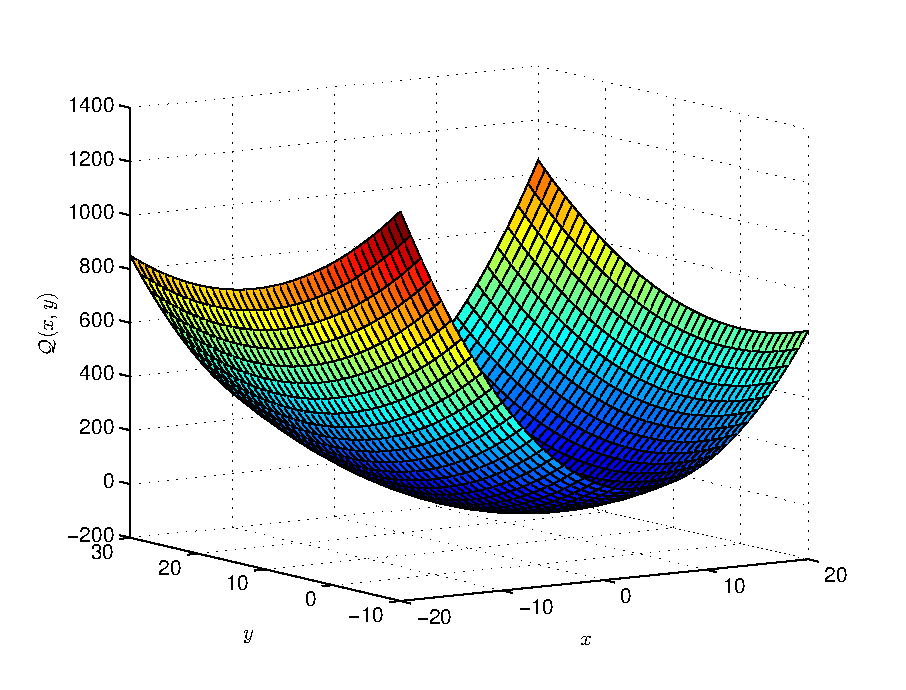
\includegraphics[scale=.7]{images/q-plot.eps}
\captionof{figure}{අභ්‍යාන්තරික සාන්දර්භය}
\label{fig:graph}
\end{center}

 දෙවියන්වහන්සේ ඔවුන්ට කියනසේක්: නුඹලා බෝවී වැඩිවෙමින් පොළොව පූර්ණකොට ඒක යටත්කරගනිව්; මුහුදේ මත්ස්‍යයන් කෙරෙහිද ආකාශයේ පක්ෂීන් කෙරෙහිද පොළොව පිට හැසිරෙන සියලු සතුන් කෙරෙහිද අධිපතිකම් කරව්යයි කීසේක. 29තවද දෙවියන්වහන්සේ: බලව, මුළු පොළෝතලයෙහි ඇති බීජ දරන සියලු පලාද බීජ දරන ඵල ඇති සියලු වෘක්ෂයන්ද නුඹලාට දුනිමි; එය නුඹලාට ආහාර පිණිස වන්නේය. 30පොළොවේ සියලු මෘගයන්ටත් ආකාශයේ සියලු පක්ෂීන්ටත් පොළොව පිට බඩගා යන පණ ඇති (සියලු සතුන්ටත් ආහාර පිණිස) (test)සියලු නිල් පලා දුනිමියි කීසේක. ඒ එසේ විය. 31දෙවියන්වහන්සේ තමන් සෑදූ සියල්ලම දුටුසේක, බලව ඒ ඉතා යහපත්ව තිබුණේය. සවස විය, උදය විය, ඒ සවෙනි දවසක්ය. 

 
\end{document}  